\documentclass[12pt]{beamer}
\usepackage{../Estilos/BeamerFC}
\usepackage{../Estilos/ColoresLatex}
\usepackage{courier}
\usepackage{listingsutf8}
\usepackage{listings}
\usepackage{xcolor}
\usepackage{textcomp}
\usepackage{color}
\definecolor{deepblue}{rgb}{0,0,0.5}
\definecolor{brown}{rgb}{0.59, 0.29, 0.0}
\definecolor{OliveGreen}{rgb}{0,0.25,0}
% \usepackage{minted}

\DeclareCaptionFont{white}{\color{white}}
\DeclareCaptionFormat{listing}{\colorbox{gray}{\parbox{0.98\textwidth}{#1#2#3}}}
\captionsetup[lstlisting]{format=listing,labelfont=white,textfont=white}
\renewcommand{\lstlistingname}{Código}


\definecolor{Code}{rgb}{0,0,0}
\definecolor{Keywords}{rgb}{255,0,0}
\definecolor{Strings}{rgb}{255,0,255}
\definecolor{Comments}{rgb}{0,0,255}
\definecolor{Numbers}{rgb}{255,128,0}

\makeatletter

\newif\iffirstchar\firstchartrue
\newif\ifstartedbyadigit
\newif\ifprecededbyequalsign

\newcommand\processletter
{%
  \ifnum\lst@mode=\lst@Pmode%
    \iffirstchar%
        \global\startedbyadigitfalse%
      \fi
      \global\firstcharfalse%
    \fi
}

\newcommand\processdigit
{%
  \ifnum\lst@mode=\lst@Pmode%
      \iffirstchar%
        \global\startedbyadigittrue%
      \fi
      \global\firstcharfalse%
  \fi
}

\lst@AddToHook{OutputOther}%
{%
  \lst@IfLastOtherOneOf{=}
    {\global\precededbyequalsigntrue}
    {}%
}

\lst@AddToHook{Output}%
{%
  \ifprecededbyequalsign%
      \ifstartedbyadigit%
        \def\lst@thestyle{\color{orange}}%
      \fi
    \fi
  \global\firstchartrue%
  \global\startedbyadigitfalse%
  \global\precededbyequalsignfalse%
}

\lstset{ 
language=Python,                % choose the language of the code
basicstyle=\footnotesize\ttfamily,       % the size of the fonts that are used for the code
numbers=left,                   % where to put the line-numbers
numberstyle=\scriptsize,      % the size of the fonts that are used for the line-numbers
stepnumber=1,                   % the step between two line-numbers. If it is 1 each line will be numbered
numbersep=5pt,                  % how far the line-numbers are from the code
backgroundcolor=\color{white},  % choose the background color. You must add \usepackage{color}
showspaces=false,               % show spaces adding particular underscores
showstringspaces=false,         % underline spaces within strings
showtabs=false,                 % show tabs within strings adding particular underscores
frame=single,   		% adds a frame around the code
tabsize=2,  		% sets default tabsize to 2 spaces
captionpos=t,   		% sets the caption-position to bottom
breaklines=true,    	% sets automatic line breaking
breakatwhitespace=false,    % sets if automatic breaks should only happen at whitespace
escapeinside={| |},  % if you want to add a comment within your code
stringstyle =\color{OliveGreen},
otherkeywords={as, np.array, np.concatenate, np.linspace, linspace, interpolate.interp1d, kind, plt.plot, .copy, np.arange, np.cos, np.pi, lw, ls, label, splrep, splev, plt.legend, loc, plt.title, plt.ylim, plt.show, sign, math.ceil, math.log, np.sqrt, np.exp, np.zeros, plt.xlabel, plt.ylabel, plt.xlim, np.identity, random, np.dot, np.outer, np.diagonal },             % Add keywords here
keywordstyle = \color{blue},
commentstyle = \color{darkcerulean},
identifierstyle = \color{black},
literate=%
         {á}{{\'a}}1
         {é}{{\'e}}1
         {í}{{\'i}}1
         {ó}{{\'o}}1
         {ú}{{\'u}}1
%
%keywordstyle=\ttb\color{deepblue}
%fancyvrb = true,
}

\lstdefinestyle{FormattedNumber}{%
    literate={0}{{\textcolor{red}{0}}}{1}%
             {1}{{\textcolor{red}{1}}}{1}%
             {2}{{\textcolor{red}{2}}}{1}%
             {3}{{\textcolor{red}{3}}}{1}%
             {4}{{\textcolor{red}{4}}}{1}%
             {5}{{\textcolor{red}{5}}}{1}%
             {6}{{\textcolor{red}{6}}}{1}%
             {7}{{\textcolor{red}{7}}}{1}%
             {8}{{\textcolor{red}{8}}}{1}%
             {9}{{\textcolor{red}{9}}}{1}%
             {.0}{{\textcolor{red}{.0}}}{2}% Following is to ensure that only periods
             {.1}{{\textcolor{red}{.1}}}{2}% followed by a digit are changed.
             {.2}{{\textcolor{red}{.2}}}{2}%
             {.3}{{\textcolor{red}{.3}}}{2}%
             {.4}{{\textcolor{red}{.4}}}{2}%
             {.5}{{\textcolor{red}{.5}}}{2}%
             {.6}{{\textcolor{red}{.6}}}{2}%
             {.7}{{\textcolor{red}{.7}}}{2}%
             {.8}{{\textcolor{red}{.8}}}{2}%
             {.9}{{\textcolor{red}{.9}}}{2}%
             {\ }{{ }}{1}% handle the space
         ,%
          %mathescape=true
          escapeinside={__}
          }



\usepackage[siunitx]{circuitikz}
\usetikzlibrary{arrows,patterns,shapes}
\usetikzlibrary{decorations.markings}
\usetikzlibrary{arrows}
\usetheme{Copenhagen}
\usecolortheme{wolverine}
%\useoutertheme{default}
\setbeamercovered{invisible}
% or whatever (possibly just delete it)
\setbeamertemplate{section in toc}[sections numbered]
\setbeamertemplate{subsection in toc}[subsections numbered]
\setbeamertemplate{subsection in toc}{\leavevmode\leftskip=3.2em\rlap{\hskip-2em\inserttocsectionnumber.\inserttocsubsectionnumber}\inserttocsubsection\par}
% \setbeamercolor{section in toc}{fg=blue}
% \setbeamercolor{subsection in toc}{fg=blue}
% \setbeamercolor{frametitle}{fg=blue}
\setbeamertemplate{caption}[numbered]

\setbeamertemplate{footline}
\beamertemplatenavigationsymbolsempty
\setbeamertemplate{headline}{}


\makeatletter
% \setbeamercolor{section in foot}{bg=gray!30, fg=black!90!orange}
% \setbeamercolor{subsection in foot}{bg=blue!30}
% \setbeamercolor{date in foot}{bg=black}
\setbeamertemplate{footline}
{
  \leavevmode%
  \hbox{%
  \begin{beamercolorbox}[wd=.333333\paperwidth,ht=2.25ex,dp=1ex,center]{section in foot}%
    \usebeamerfont{section in foot} \insertsection
  \end{beamercolorbox}%
  \begin{beamercolorbox}[wd=.333333\paperwidth,ht=2.25ex,dp=1ex,center]{subsection in foot}%
    \usebeamerfont{subsection in foot}  \insertsubsection
  \end{beamercolorbox}%
  \begin{beamercolorbox}[wd=.333333\paperwidth,ht=2.25ex,dp=1ex,right]{date in head/foot}%
    \usebeamerfont{date in head/foot} \insertshortdate{} \hspace*{2em}
    \insertframenumber{} / \inserttotalframenumber \hspace*{2ex} 
  \end{beamercolorbox}}%
  \vskip0pt%
}
\makeatother

\makeatletter
\patchcmd{\beamer@sectionintoc}{\vskip1.5em}{\vskip0.8em}{}{}
\makeatother

% %\newlength{\depthofsumsign}
% \setlength{\depthofsumsign}{\depthof{$\sum$}}
% \newcommand{\nsum}[1][1.4]{% only for \displaystyle
%     \mathop{%
%         \raisebox
%             {-#1\depthofsumsign+1\depthofsumsign}
%             {\scalebox
%                 {#1}
%                 {$\displaystyle\sum$}%
%             }
%     }
% }
% \def\scaleint#1{\vcenter{\hbox{\scaleto[3ex]{\displaystyle\int}{#1}}}}
% \def\scaleoint#1{\vcenter{\hbox{\scaleto[3ex]{\displaystyle\oint}{#1}}}}
% \def\bs{\mkern-12mu}

% \usefonttheme{serif}

\title{\large{Solución de EDO con python}}
\subtitle{Tema 3 - Ecuaciones Diferenciales Ordinarias}
\author{M. en C. Gustavo Contreras Mayén}
\date{}

\begin{document}
\maketitle

\section{python para resolver las EDO}
\frame{\tableofcontents[currentsection, hideothersubsections]}
\subsection{Antes de usar la librería}

\begin{frame}
\frametitle{Usando \python{} para resolver las EDO}
Un sistema de EDOs se escribe en la forma estándar antes de ser resuelto numéricamente con \python.
\end{frame}
\begin{frame}
\frametitle{Usando \python{} para resolver las EDO}
La forma estándar es:
\begin{align*}
\pderivada{y} = f (y, t)
\end{align*}
\pause
donde:
\pause
\begin{align*}
y = [y_{1} (t), y_{2} (t), \ldots, y _{n} (t)]
\end{align*}
y $f$ es una función que determina las derivadas de la función $y_{i} (t)$.
\end{frame}
\begin{frame}
\frametitle{Usando \python{} para resolver las EDO}
Para resolver la EDO necesitamos conocer la función $f$ y una condición inicial: $y (0)$.
\\
\medskip
\pause
Ya revisamos que las EDO de orden superior siempre se pueden escribir en la forma estándar, introduciendo para ello nuevas variables para las derivadas intermedias.
\end{frame}
\section{La función \texttt{odeint}}
\begin{frame}
\frametitle{La función \texttt{scipy.integrate.odeint}}
Dentro del módulo \funcionazul{scipy.integrate} tenemos disponible la función \funcionazul{odeint}, que integra un sistema de EDO.
\pause
\begin{align*}
\dv{y}{t} = \mbox{ func}(y, t_{0}, ...)
\end{align*}
donde $y$ puede ser un vector.
\end{frame}
\begin{frame}[fragile]
\frametitle{La sintaxis para \texttt{odeint}}
La sintaxis básica para la función es la siguiente:
\\
\bigskip
\pause
\funcionazul{odeint(func, y0, t, args=())}
\end{frame}
\begin{frame}
\frametitle{Los parámetros de \texttt{odeint}}
Los parámetros son los siguientes:
\setbeamercolor{item projected}{bg=cerise,fg=bananayellow}
\setbeamertemplate{enumerate items}{%
\usebeamercolor[bg]{item projected}%
\raisebox{1.5pt}{\colorbox{bg}{\color{fg}\footnotesize\insertenumlabel}}%
}
\begin{enumerate}[<+->]
\item \funcionazul{func} : Función que se manda llamar $(y, t0, ...)$ Calcula la derivada de $y$ en $t_{0}$.
\item \funcionazul{y0} : arreglo. Condición inicial de $y$, puede ser un vector.
\seti
\end{enumerate}
\end{frame}
\begin{frame}
\frametitle{Los parámetros de \texttt{odeint}}
\setbeamercolor{item projected}{bg=cerise,fg=bananayellow}
\setbeamertemplate{enumerate items}{%
\usebeamercolor[bg]{item projected}%
\raisebox{1.5pt}{\colorbox{bg}{\color{fg}\footnotesize\insertenumlabel}}%
}
\begin{enumerate}[<+->]
\conti
\item \funcionazul{t} : arreglo. Una secuencia de puntos temporales en los cuales se va a resolver para la variable $y$. La condición inicial debe de ser el primer elemento de esta secuencia.
\item \funcionazul{args} : tupla opcional. Argumentos extra para pasar a la función.
\end{enumerate}
\end{frame}
\begin{frame}
\frametitle{Lo que devuelve la función \textbf{odeint}}
La función \funcionazul{odeint} devuelve una serie de elementos, el principal es:
\\
\medskip
\pause
$y$ : arreglo, \texttt{shape (len(t), len(y0))}
\\
\medskip
Que es un arreglo que contiene los valores de $y$ para cada punto temporal $t$, con la condición inicial $y_{0}$ en el primer renglón.
\end{frame}
\begin{frame}
\frametitle{Usando la función \texttt{odeint}}
Una vez definida la función $F$ y el arreglo $y_{0}$, podemos usar la función \funcionazul{odeint}:
\pause
\begin{align*}
y_{t} = \mbox{\texttt{odeint}} (F, y_{0}, t)
\end{align*}
Nótese que contiene el mínimo de argumentos para la función.
\end{frame}

\subsection{Ejercicios con \texttt{odeint}}

\begin{frame}
\frametitle{Ejercicio 1 - Péndulo con fricción}
La \funcionazul{EDO2} para el ángulo $\theta$ de un péndulo que se desplaza bajo la acción de la gravedad y con fricción, se puede escribir como:
\pause
\begin{align*}
\ddot{\theta} +  b \: \dot{\theta} +  c \: \sin \theta = 0 
\end{align*}
donde $b$ y $c$ son constantes positivas.
\end{frame}
\begin{frame}
\frametitle{Solución al ejercicio}
Para resolver el problema con la función \funcionazul{odeint} debemos convertir a un sistema de \funcionazul{EDO1}.
\\
\bigskip
\pause
Definiendo la velocidad angular $\omega (t) = \dot{\theta}$, se obtiene el sistema:
\pause
\begin{align*}
\dot{\theta} &= \omega \\
\dot{\omega} &= -b \:\omega - c \: \sin(\theta)
\end{align*}
\end{frame}
\begin{frame}[fragile]
\frametitle{Solución al ejercicio}
Sea el vector $y =  [\theta, \omega]$. Así la función que usaremos en \python{} queda como:
\begin{lstlisting}[caption=Función a integrar para el ejecicio del péndulo]
def F(y, t, b, c):
    theta, omega = y
    dydt = [omega, -b * omega - c * np.sin(theta)]
    return dydt
\end{lstlisting}
\end{frame}
\begin{frame}
\frametitle{Valores de las constantes}
Consideramos que las constantes $b$ y $c$ son:
\begin{align*}
b &= 0.25 \\
c &= 5.0
\end{align*} 
\end{frame}
\begin{frame}
\frametitle{Condiciones inciales}
Para las condiciones iniciales, supongamos que el péndulo está muy cerca de la vertical con $\theta(0) = \pi - 0.1$, y que está en reposo, por lo que $\omega(0) = 0$.
\\
\bigskip
\pause
Entonces, el vector de las condiciones iniciales queda como:
\pause
\begin{align*}
y0 =  [\pi - 0.1 , \; 0.0]
\end{align*}
\end{frame}
\begin{frame}
\frametitle{Secuencia temporal}
Generamos una secuencia de $101$ puntos temporales en el intervalo $0 \leq t \leq 10$, por lo que nuestro arreglo de tiempo es:
\pause
\begin{align*}
t =  \mbox{\texttt{np.linspace}}(0., \; 10., \; 101)
\end{align*}
\end{frame}
\begin{frame}[fragile]
\frametitle{Solución con \texttt{odeint}}
Usamos la función \funcionazul{odeint} para la solución; el paso de los parámetros $b$ y $c$ a \funcionazul{F}, se hace a través de \funcionazul{args}:
\pause
\begin{lstlisting}[caption=Solución con odeint]
from scipy.integrate import odeint

sol = odeint(F, y0, t, args=(b, c))
\end{lstlisting}
\end{frame}
\begin{frame}[plain, allowframebreaks, fragile]
\frametitle{Código completo}
\begin{lstlisting}[caption=Función con las EDO1 a integrar]
from scipy.integrate import odeint
import matplotlib.pyplot as plt
import numpy as np

def F(y, t, b, c):
    theta, omega = y
    dydt = [omega, -b * omega - c * np.sin(theta)]
    return dydt

b = 0.25
c = 5.0

y0 =  [np.pi - 0.1, 0.0]

t = np.linspace(0., 10., 101)

sol = odeint(F, y0, t, args=(b, c))

# Agregamos las rutinas de graficacion
\end{lstlisting}
\end{frame}
\begin{frame}[plain]
\frametitle{Gráficas de la solución}
La gráfica muestra la posición y la velocidad angular del péndulo.
\begin{figure}
    \centering
    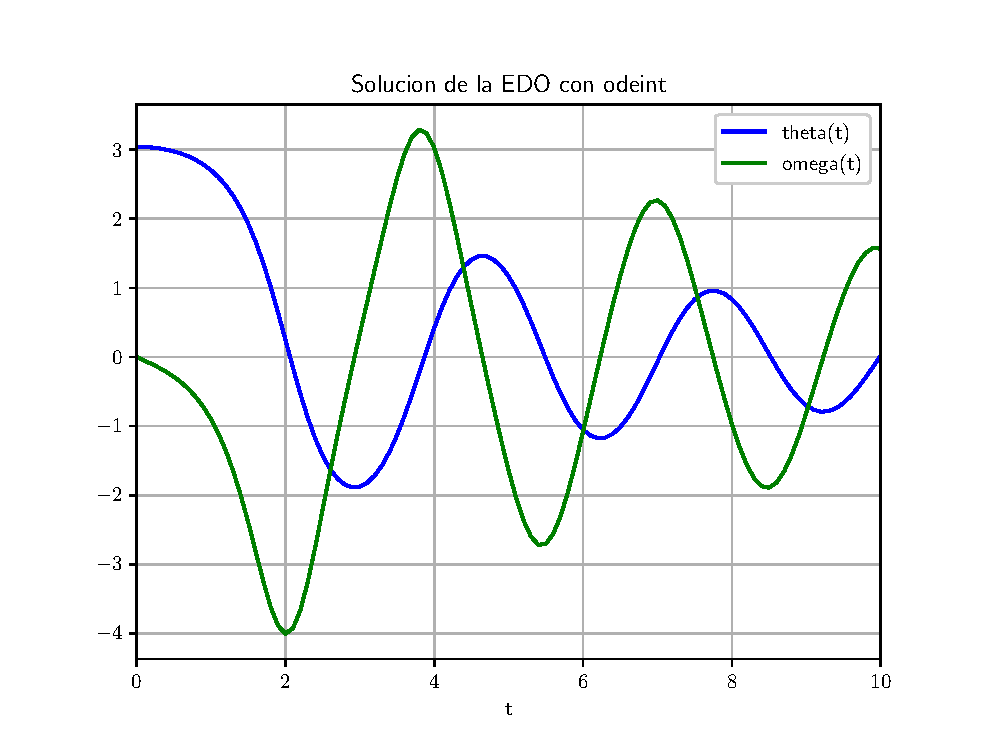
\includegraphics[scale=0.5]{Imagenes/plot_Ejercicio_odeint_01_Pendulo.eps}
\end{figure}
\end{frame}
\begin{frame}[plain]
\frametitle{Gráfica del espacio fase}
Encontramos un atractor debido a la fricción en el péndulo.
\begin{figure}
    \centering
    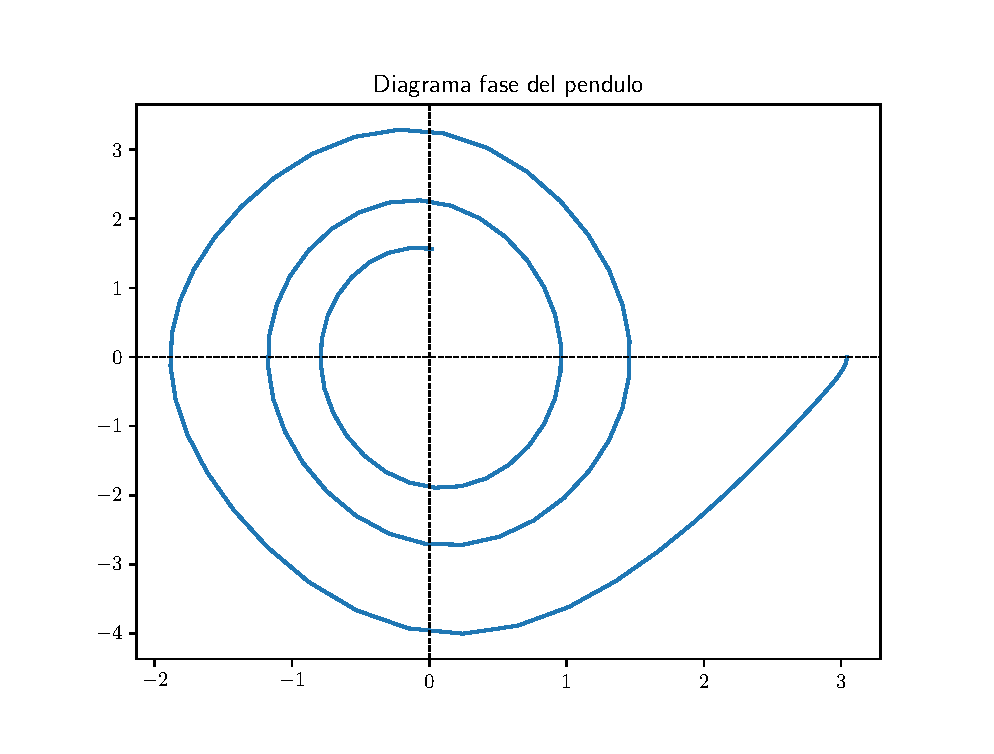
\includegraphics[scale=0.5]{Imagenes/plot_Ejercicio_odeint_02_Pendulo.eps}
\end{figure}
\end{frame}

\begin{frame}
\frametitle{Ejercicio 2 - Oscilador amortiguado}
La ecuación de movimiento para el oscilador amortiguado es:
\pause
\begin{align*}
\dv[2]{x}{t} + 2 \: \zeta \:  \omega_{0} \, \dv{x}{t} + \omega_{0}^{2} \: x = 0
\end{align*}
donde $x$ es la posición del oscilador, $\omega_{0}$ la frecuencia, y $\zeta$ es el factor de amortiguamiento.
\end{frame}
\begin{frame}
\frametitle{Re-escribiendo la EDO}
Para escribir esta \funcionazul{EDO2} en la forma estándar, introducimos $p = \dv*{x}{t}$:
\pause
\begin{align*}
\dv{p}{t} &= - 2 \: \zeta \: \omega_{0} \: p - \omega^{2} \: x \\
\dv{x}{t} &= p
\end{align*}
\end{frame}
\begin{frame}
\frametitle{Usando argumentos}
Veremos con este ejemplo, la versatilidad de pasar argumentos extras a la función, que representan diferentes valores del factor de amortiguamiento.
\end{frame}
\begin{frame}
\frametitle{Usando argumentos}
De tal manera que en una sola ejecución del código, podemos realizar el pase de valores, \pause de otra manera, tendríamos que realizar una ejecución del código y modificar a mano el valor del factor de amortiguamiento.
\end{frame}
\begin{frame}
\frametitle{Usando argumentos}
Debido a los argumentos extra, necesitamos pasar un argumento clave \funcionazul{args} a la función \funcionazul{odeint}.
\pause
\begin{align*}
\zeta = 0.0, 0.2, 1.0, 5.0
\end{align*}
\end{frame}
\begin{frame}[plain, allowframebreaks, fragile]
\frametitle{Código para resolver el problema}
\begin{lstlisting}[caption=Código completo para el oscilador amortiguado]
from scipy.integrate import odeint
from numpy import zeros, array, linspace
import matplotlib.pyplot as plt

def F(y, t, zeta, w0):
    F = zeros((2), dtype='float64')
    F[0] = y[1]
    F[1] = -2 * zeta * w0 * y[1] - w0**2 * y[0]
    return F    

y0 =array([1.0, 0.0])

t = linspace(0, 10, 1000)
w0 = 2 * pi * 1.0

y1 = odeint(F, y0, t, args=(0.0, w0))
y2 = odeint(F, y0, t, args=(0.2, w0))
y3 = odeint(F, y0, t, args=(1.0, w0))
y4 = odeint(F, y0, t, args=(5.0, w0))

# Aqui va la rutina de graficacion
\end{lstlisting}
\end{frame}
\begin{frame}
\frametitle{Gráfica con las soluciones}
\begin{figure}
    \centering
    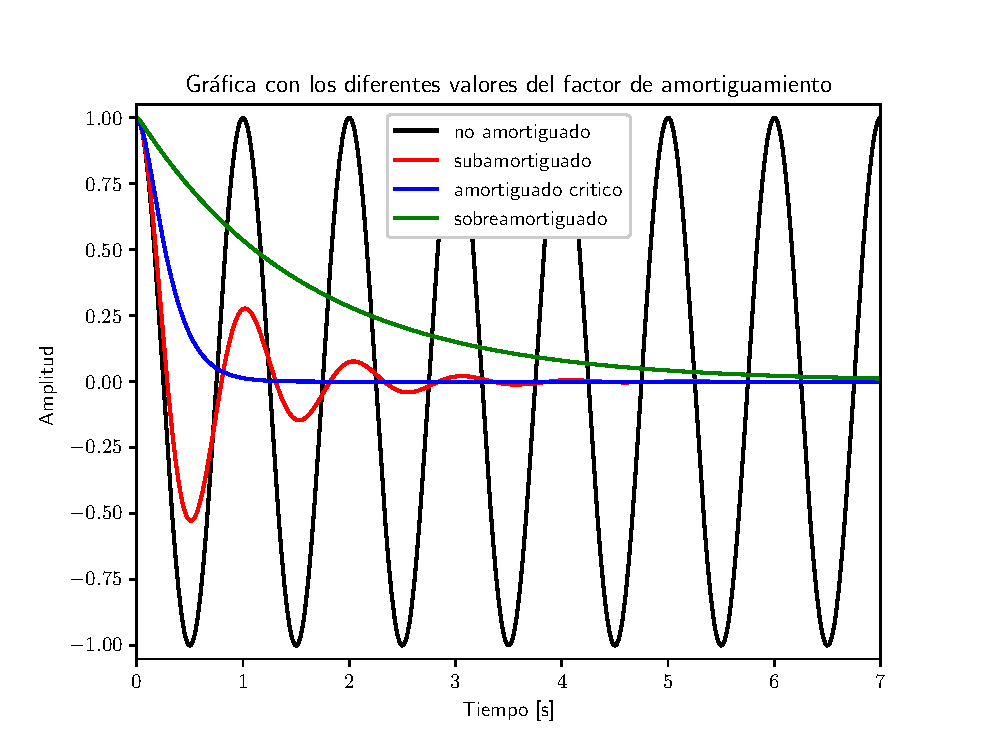
\includegraphics[scale=0.55]{Imagenes/plot_Ejercicio_odeint_02_Pendulo_Casos.eps} 
\end{figure}
\end{frame}

\begin{frame}
\frametitle{Ejercicio 3 - Circuito RLC}
La corriente eléctrica de un circuito $RLC$ en serie:
\begin{figure}
    % \centering
    % \includegraphics[scale=1]{Imagenes/fig_edo_cto_RLC.eps}
    \begin{circuitikz}
	\draw
	    (0,0)
	        to[sV, l=$V_{s}$] ++(0,3)
	        to[short] ++(1,0)
	        to[cspst, o-o] ++(1,0)
	        to[short] ++(1,0)
	        to[L, l=$L$] ++(1,0)
	        to[short] ++(1,0)
	        to[short] ++(0,-1)
	        to[C, l=$C$] ++(0,-1)
	        to[short] ++(0,-1)
	        to[short] ++(-1,0)
	        to[R, l=$R$] ++(-1,0) --(0,0);
	\end{circuitikz}
\end{figure}
\end{frame}
\begin{frame}
\frametitle{EDO del circuito RLC}
Satisface la ecuación:
\pause
\begin{equation} \label{eq:ecuacion1}
L \, \dv{i}{t} + R \: i+ \dfrac{1}{C} \scaleint{6ex}_{\bs 0}^{t} i (\pderivada{t}) \dd{\pderivada{t}} +\dfrac{1}{C} \: q(0) = E(t), \hspace{0.3cm} t > 0 
\end{equation}
\end{frame}
\begin{frame}
\frametitle{Circuito RLC}
Cuando el circuito se cierra en el instante $t = 0$, se tiene que $i = i(t)$ es la corriente, $R$ es la resistencia, $L, C, E$ vienen dadas por:
\begin{itemize}
\item $L = \SI{200}{\henry}$
\item $C = \SI{0.001}{\farad}$
\item $E(t) = \SI{1}{\volt}$ para $t > 0$.
\end{itemize}
\end{frame}
\begin{frame}
\frametitle{Circuito RLC}
\begin{figure}
    \centering
    % \includegraphics[scale=0.7]{Imagenes/fig_edo_cto_RLC.eps}
    \begin{circuitikz}
        \draw
            (0,0)
                to[sV, l=$V_{s}$] ++(0,3)
                to[short] ++(1,0)
                to[cspst, o-o] ++(1,0)
                to[short] ++(1,0)
                to[L, l=$L$] ++(1,0)
                to[short] ++(1,0)
                to[short] ++(0,-1)
                to[C, l=$C$] ++(0,-1)
                to[short] ++(0,-1)
                to[short] ++(-1,0)
                to[R, l=$R$] ++(-1,0) --(0,0);
        \end{circuitikz}
\end{figure}
Las condiciones iniciales son $q (0) = 0$ (carga inicial del condensador), $i (0) = 0$. 
\end{frame}
\begin{frame}
\frametitle{Resolver el problema}
Calcula la corriente para $0 \leq t \leq 5$ segundos y el factor de amortiguamiento y la frecuencia de oscilación del circuito $RLC$ para los siguientes valores de R:
\pause
\setbeamercolor{item projected}{bg=black,fg=white}
\setbeamertemplate{enumerate items}{%
\usebeamercolor[bg]{item projected}%
\raisebox{1.5pt}{\colorbox{bg}{\color{fg}\footnotesize\insertenumlabel}}%
}
\begin{enumerate}[<+->]
\item $R = \SI{0}{\ohm}$
\item $R = \SI{50}{\ohm}$
\item $R = \SI{100}{\ohm}$
\item $R = \SI{300}{\ohm}$
\end{enumerate}
\end{frame}
\begin{frame}
\frametitle{Manejando las expresiones}
Si definimos:
\pause
\begin{equation}\label{eq:ecuacion2}
q (t) = \scaleint{6ex}_{\bs 0}^{\pderivada{t}} i (\pderivada{t}) \: \dd{\pderivada{t}}
\end{equation}
\pause
derivando la expresión anterior:
\pause
\begin{equation}\label{eq:ecuacion3}
\dv{t} \, q(t) = i (t), \hspace{1.5cm} q (0) = 0
\end{equation}
\end{frame}
\begin{frame}
\frametitle{Sustituyendo las expresiones}
Sustituimos en la ecuación inicial, para reescribir:
\pause
\begin{equation}\label{eq:ecuacion4}
\dv{t} i (t) = -\dfrac{R}{L} \: i (t) - \dfrac{1}{L \: C} \: q(t) + \dfrac{1}{L \: C} \: q(0) + \dfrac{E (t)}{L}, \: i(0) =  0 
\end{equation}
La ecuación (\ref{eq:ecuacion1}) se transformó en un sistema de dos EDO1: las ecuaciones (\ref{eq:ecuacion3}) y (\ref{eq:ecuacion4}).
\end{frame}
\begin{frame}[fragile, allowframebreaks]
\begin{lstlisting}[caption=Código para el circuito RLC]
from numpy import zeros, array, linspace
from scipy.integrate import odeint
import matplotlib.pyplot as plt

def F(y, t, R, L) : 
    C = 0.001
    E = 1.0
            
    F = zeros(2)
    F[0] = y[1]
    F[1] = -(R/L) * y[1] - (1.0/(L * C)) * y[0] + E/L
    return F

t = linspace(0.0, 5.0, 100)
y0 = array([0., 0.])

L = 200.0
R = [0., 50, 100, 300]

sol = odeint(F, y0, t)

# Hay que ajustar el codigo para que en un solo paso
# se tengan las cuatro graficas en una sola imagen
\end{lstlisting}
\end{frame}
\begin{frame}
\frametitle{Solución gráfica con valores de $R$ superpuestos}
\begin{figure}
    \centering
    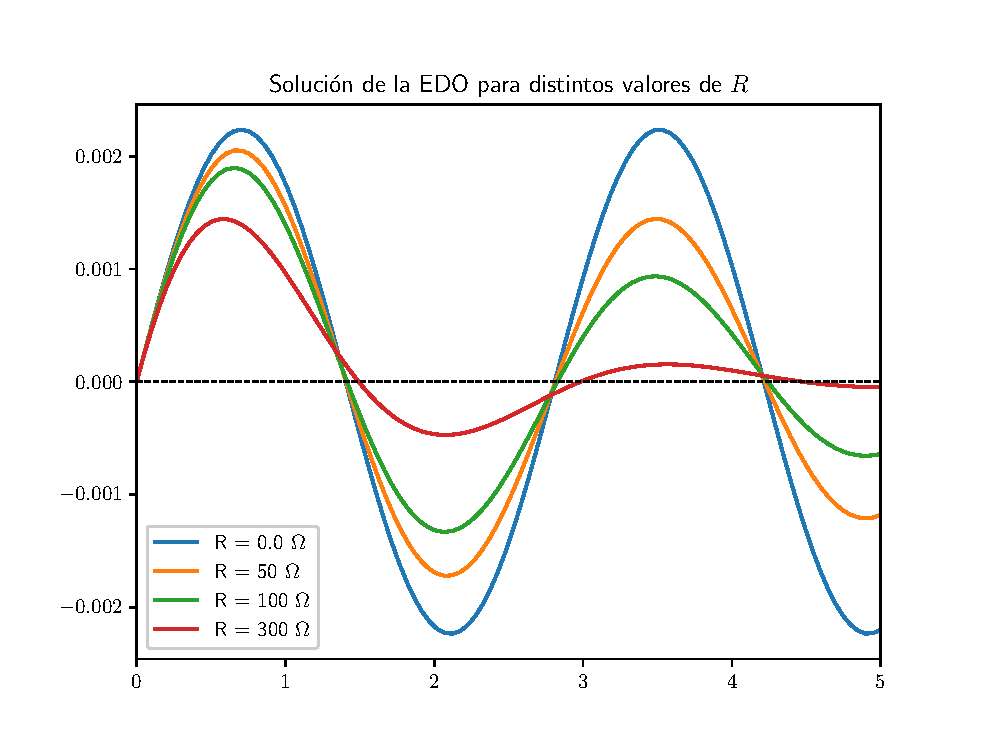
\includegraphics[scale=0.55]{Imagenes/plot_Ejercicio_odeint_03_Circuito_RLC.eps}
\end{figure}
\end{frame}
% \subsection{Sistema de 3 masas acopladas}
% \begin{frame}[fragile]
% \frametitle{Ejercicio 4 - Masas acopladas}
% En la figura se muestra un sistema de tres masas acopladas mediante resortes y amortiguadores.
% \begin{figure}
%     \centering
%     \includestandalone[scale=0.75]{Figuras/fig_edo_sist_3_masas}
% \end{figure}
% \end{frame}
% \begin{frame}[fragile]
% \frametitle{Ejercicio 4 - Masas acopladas}
% Los desplazamientos de estas tres masas satisfacen las ecuaciones dadas por:
% \fontsize{12}{12}\selectfont
% \begin{align*} 
%     M_{1} \: y^{\prime \prime}{1} + B_{1} \: y^{\prime}_{1} + K_{1} \: y_{1} - B_{1} \: y^{\prime}_{2} - K_{2} \: y_{2} & = F_{1}(t) \\
%     -B_{1} \: y^{\prime}_{1} - K_{1} \: y_{1} + M_{2} \:  y^{\prime \prime}_{2} + B_{1} \: y^{\prime}_{2} + (K_{1} + K_{2}) \: y_{2} - K_{2} \: y_{3} & = 0 \\
%     - K_{2} \: y_{2} + M_{3} \: y^{\prime \prime}_{3} + B_{2} \: y^{\prime}_{3} + (K_{2} + K_{3})  \: y_{3} & =  F_{3}(t) 
% \end{align*}
% \begin{figure}
%     \centering
%     \includestandalone[scale=0.75]{Figuras/fig_edo_sist_3_masas}
% \end{figure}
% \end{frame}
% \begin{frame}
% \frametitle{Condiciones iniciales}
% Las constantes y condiciones iniciales son
% \fontsize{12}{12}\selectfont
% \begin{tabbing}
% $K_{1} = K_{2} = K_{3} = 1$ \hspace{1.2cm} \= (constantes de los resortes, kgm/$s^{2}$) \\
% $M_{1} = M_{2} = M_{3} = 1$ \> (masa, kg) \\
% $F_{1}(t) = 1, F_{3}(t) = 0$ \> (fuerza, N) \\
% $B_{1} = B_{2} =0.1$ \> (coeficientes de amortiguamiento, kg/s) \\
% \\
% $y_{1}(0) = y^{\prime}_{1}(0) = y_{2}(0) = y^{\prime}_{2}(0) = y_{3}(0) = y^{\prime}_{3}(0) = 0$ \\
% \> (condiciones iniciales)
% \end{tabbing}
% \end{frame}
% \begin{frame}
% \frametitle{Problema a resolver}
% Resuelve el sistema para determinar la posición $y_{i}$ de cada masa en $0 \leq t \leq 60$ segundos, elabora una gráfica con las tres trayectorias.
% \end{frame}
% \begin{frame}
% \frametitle{Antes de proponer un código}
% Necesitamos manejar el sistema de 3 EDO2, de tal manera que podamos representar un sistema de 6 EDO1, entonces consideremos el siguiente:
% \\
% \bigskip
% Hint: Definiendo
% \[ y_{4} = y^{\prime}_{1}, \hspace{1cm} y_{5} = y^{\prime}_{2}, \hspace{1cm} y_{6} = y^{\prime}_{3} \]
% \end{frame}
% \begin{frame}
% \frametitle{Antes de proponer un código}
% Así, la ecuación inicial se escribe como un conjunto de seis EDO de primer orden, de la siguiente manera:
% \fontsize{12}{12}\selectfont
% \begin{align*}
% y^{\prime}_{1} & = y_{4} \\
% y^{\prime}_{2} & = y_{5} \\
% y^{\prime}_{3} & = y_{6} \\
% y^{\prime}_{4} & = \left[ -B_{1} \: y_{4} - K_{1} \: y_{1} + B_{1} \: y_{5} + K_{2} \: y_{2} + F_{1} \right] / M_{1} \\
% y^{\prime}_{5} & = \left[ B_{1} \: y_{4} + K_{1} \: y_{1} - B_{1} \: y_{5} - \left( K_{1} + K_{2} \right) \: y_{2} + K_{2} \: y_{3} \right] / M_{2}\\
% y^{\prime}_{6} & = \left[ K_{2} \: y_{2} - B_{2} \: y_{6} - \left( K_{2} + K_{3} \right) \: y_{3} + F_{3} \right] / M_{3}
% \end{align*}
% \end{frame}
% \begin{frame}[fragile, allowframebreaks, plain]
% \begin{lstlisting}[caption=Código para el sistema de masas, style=FormattedNumber, basicstyle=\linespread{1.1}\ttfamily=\small, columns=fullflexible]
% def F(y, t) : 
%     F = zeros(6)
%     F[_0_] = y[_3_]
%     F[_1_] = y[_4_]
%     F[_2_] = y[_5_]
%     F[_3_] = (-0.1 * y[_3_]- y[_0_] + 0.1 * y[_4_] + y[_1_] + 1.)
%     F[_4_] = (0.1 * y[_3_] + y[_0_] - 0.1 * y[_4_] - 2. * y[_1_] + y[_2_])
%     F[_5_] = (y[_1_] - 0.1 * y[_5_] - 2. * y[_2_])
%     return F

% t = linspace(0, 61, 100)
% y_0_ = array([0., 0., 0., 0., 0., 0.])

% sol = odeint(F, y_0_, t)

% plt.plot(t, sol[:,_0_], label = "$M{_1_}$")
% plt.plot(t, sol[:,_1_], label = "$M{_2_}$")
% plt.plot(t, sol[:,_2_], label = "$M{_3_}$")
% plt.legend(loc='upper right')
% plt.xlabel("Tiempo [s]")
% plt.ylabel("Amplitud")
% plt.axis([0, 60, -0.5, 6])
% plt.axhline(y=0, lw=0.75, ls='dashed', color='k')
% plt.title("Sistema de tres masas")
% plt.show()
% \end{lstlisting}
% \end{frame}
% \begin{frame}[plain]
% \frametitle{Solución al problema}
% \begin{figure}
%     \centering
%     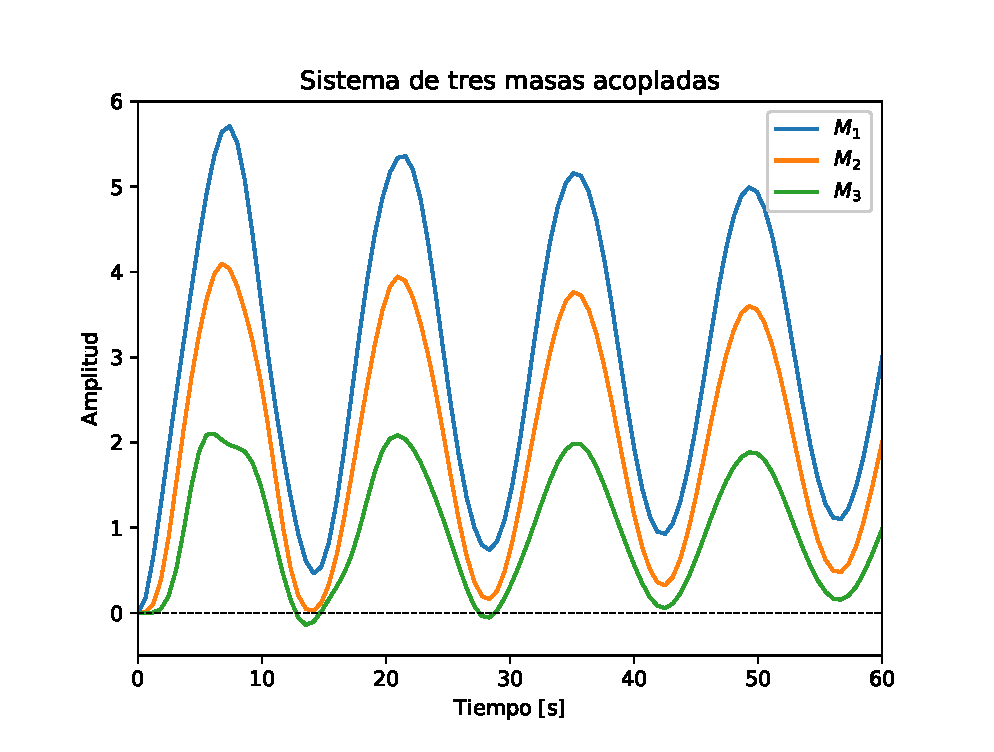
\includegraphics[scale=0.65]{SistemaTresMasasRK4.eps} 
% \end{figure}
% \end{frame}
% \subsection{Sistema Lotka-Volterra}
% \begin{frame}
% \frametitle{Sistema Lotka-Volterra}
% Las ecuaciones de Lotka-Volterra, también son conocidas como ecuaciones de depredador-presa.
% \\
% \bigskip
% Está descrito por un sistema de 2 ecuaciones diferenciales no lineales de primer orden.
% \end{frame}
% \begin{frame}
% \frametitle{Sistema Lotka-Volterra}
% Se utiliza frecuentemente para describir la dinámica de sistemas biológicos donde interaccionan dos especies: un depredador y una de sus presas.
% \end{frame}
% \begin{frame}
% \frametitle{Sistema de ecuaciones acopladas}
% El sistema evoluciona de acuerdo al par de ecuaciones:
% \begin{align*}
% \dfrac{du}{dt} &= a \: u - b \: u \: v \\
% \dfrac{dv}{dt} &= -c \: v + d \: b\: u\: v
% \end{align*}
% donde:  
% \setbeamercolor{item projected}{bg=yellow!80!black,fg=black}
% \setbeamertemplate{enumerate items}[circle]
% \begin{enumerate}[<+->]
% \item $u$ es el número de presas (ej. Conejos)
% \item $v$ es el número de depredadores (ej. Zorros)
% \seti
% \end{enumerate}
% \end{frame}
% \begin{frame}
% \frametitle{Sistema de ecuaciones acopladas}
% \begin{align*}
% \dfrac{du}{dt} &= a \: u - b \: u \: v \\
% \dfrac{dv}{dt} &= -c \: v + d \: b\: u\: v
% \end{align*}
% donde:
% \setbeamercolor{item projected}{bg=yellow!80!black,fg=black}
% \setbeamertemplate{enumerate items}[circle]
% \begin{enumerate}[<+->]
% \conti
% \item $a$ es la tasa natural de crecimiento de conejos, sin que haya zorros.
% \item $b$ es la tasa natural de la muerte de conejos, debido a la depredación.
% \seti
% \end{enumerate}
% \end{frame}
% \begin{frame}
% \frametitle{Sistema de ecuaciones acopladas}
% \begin{align*}
% \dfrac{du}{dt} &= a \: u - b \: u \: v \\
% \dfrac{dv}{dt} &= -c \: v + d \: b\: u\: v
% \end{align*}
% donde:
% \setbeamercolor{item projected}{bg=yellow!80!black,fg=black}
% \setbeamertemplate{enumerate items}[circle]
% \begin{enumerate}[<+->]
% \conti
% \item $c$ es la tasa natural de la muerte del zorro, cuando no hay conejos.
% \item $d$ es el factor que describe el número de conejos capturados.
% \end{enumerate}
% \end{frame}
% \begin{frame}
% \frametitle{Poblaciones iniciales}
% Vamos a utilizar $X = [u, v]$ para describir el estado de las poblaciones.
% \end{frame}
% \begin{frame}[plain, fragile]
% \frametitle{Definiendo las ecuaciones}
% \begin{lstlisting}[caption=Código inicial, style=FormattedNumber, basicstyle=\linespread{1.1}\ttfamily=\small, columns=fullflexible]
% from numpy import *
% import matplotlib.pyplot as plt

% a = 1.
% b = 0.1
% c = 1.5
% d = 0.75

% def dXdt(X, t = 0):
%     return array([ a * X[_0_] - b * X[_0_] * X[_1_], -c * X[_1_] + d * b * X[_0_] * X[_1_] ])
% \end{lstlisting}
% \end{frame}
% \begin{frame}[plain, fragile]
% \frametitle{Población en equilibrio}
% Antes de usar \funcionazul{odeint} para integrar el sistema, veremos de cerca la posición de equilibrio.
% \\
% \bigskip
% El equilibrio ocurre cuando la tasa de crecimiento es igual a $0$, lo que nos da dos puntos fijos:
% \begin{lstlisting}[caption=Equilibrio en las poblaciones, style=FormattedNumber, basicstyle=\linespread{1.1}\ttfamily=\small, columns=fullflexible]
% Xf_0_ = array([0., 0.])
% Xf_1_ = array([ c/(d * b), a/b])
% all(dXdt(Xf_0_) == zeros(_2_) ) and all(dXdt(Xf1) == zeros(_2_))
% \end{lstlisting}
% \end{frame}
% \begin{frame}[fragile]
% \frametitle{Variable temporal y cond. iniciales}
% Para usar la función \funcionazul{odeint}, hay que definir el parámetro de tiempo $t$, así como las condiciones inciales de la población: $10$ conejos y $5$ zorros.
% \end{frame}
% \begin{frame}[fragile]
% \frametitle{Variable temporal y cond. iniciales}
% \begin{lstlisting}[caption=Código para las condiciones iniciales, style=FormattedNumber, basicstyle=\linespread{1.1}\ttfamily=\small, columns=fullflexible]
% t = linspace(0, 15,  1000)
              
% X_0_ = array([10, 5])         
            
% X = integrate.odeint(dXdt, X_0_, t)
% \end{lstlisting}
% \end{frame}
% \begin{frame}
% \frametitle{Graficando la solución}
% Una vez obtenido el código para la solución del problema, ahora nos corresponde graficar el conjunto de datos obtenido:
% \end{frame}
% \begin{frame}[fragile, plain, allowframebreaks]
% \frametitle{Graficando la solución}
% \begin{lstlisting}[caption=Código para graficar, style=FormattedNumber, basicstyle=\linespread{1.1}\ttfamily=\small, columns=fullflexible]
% conejos, zorros = X.T

% f_1_ = plt.figure()
% plt.plot(t, conejos, 'r-', label='Conejos')
% plt.plot(t, zorros  , 'b-', label='Zorros')
% plt.grid()
% plt.legend(loc='best')
% plt.xlabel('tiempo')
% plt.ylabel('poblacion')
% plt.title('Evolucion de la poblacion de conejos y zorros')
% plt.show()
% \end{lstlisting}
% \end{frame}
% \begin{frame}[plain]
% \frametitle{Resultado gráfico}
% \begin{figure}
%     \centering
%     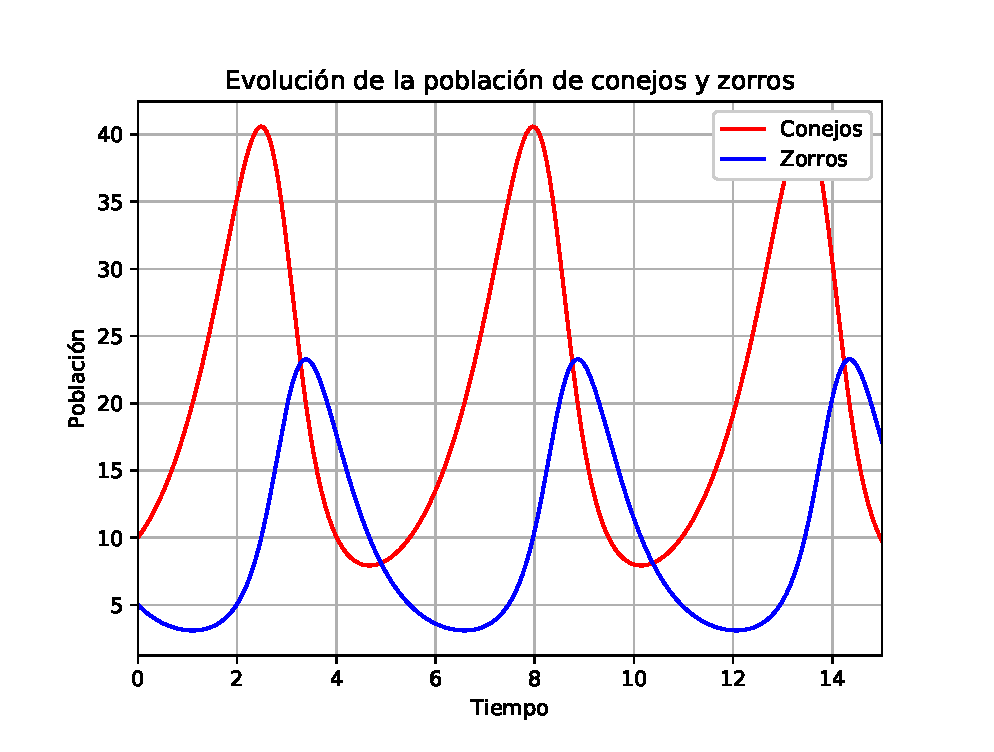
\includegraphics[scale=0.6]{Imagenes/LotkaVolterra_01.eps} 
% \end{figure}
% \end{frame}
% \begin{frame}
% \frametitle{Primer resultado}
% La gráfica anterior nos da la información sobre el número tanto de conejos como de zorros durante el intervalo de tiempo estudiado, es decir, tenemos una especie de \enquote{censo}.
% \\
% \medskip
% Para ver la dinámica de las poblaciones propiamente, ahora representamos el espacio fase del sistema, por lo que tenemos que hacer algunos ajustes en el código que usamos anteriormente.
% \end{frame}
% \begin{frame}[fragile]
% \frametitle{Condiciones de equilibrio}
% Consideremos las condiciones de equilibrio, es decir, donde la tasa de crecimiento es cero:
% \begin{lstlisting}[caption=Condiciones de equilibrio, style=FormattedNumber, basicstyle=\linespread{1.1}\ttfamily=\small, columns=fullflexible]
% Xf_0_ = array([0. , 0.])
% Xf_1_ = array([ c/(d * b), a/b])
% \end{lstlisting}
% \end{frame}
% \begin{frame}[fragile]
% \frametitle{Elementos adicionales para la gráfica}
% Dibujaremos el espacio fase con algunos elementos visuales con el fin de decoración nada más.
% \begin{lstlisting}[caption=Obteniendo los colores, style=FormattedNumber, basicstyle=\linespread{1.1}\ttfamily=\small, columns=fullflexible]
% values  = linspace(0.3, 0.9, 5)                         

% vcolors = plt.cm.autumn_r(linspace(0.3, 1., len(values)))  

% f2 = plt.figure()
% \end{lstlisting}
% \end{frame}
% \begin{frame}[fragile]
% \frametitle{El módulo \texttt{color map}}
% El módulo \funcionazul{cm} proporciona un conjunto de mapas de colores predeterminados, así como las funciones necesarias para crear nuevos mapas de color.
% \end{frame}
% \begin{frame}[fragile]
% \frametitle{El módulo \texttt{color map}}
% Existen varios mapas ya definidos: \funcionazul{autumn, bone, cool, copper, flag, gray, hot, hsv, jet, pink, prism, spring, summer, winter, spectral}.
% \end{frame}
% \begin{frame}[plain, fragile]
% \frametitle{Curvas de nivel}
% Se van a dibujar ahora las trayectorias para diferentes condiciones iniciales (número de conejos y zorros)
% \begin{lstlisting}[caption=Graficando las curvas de nivel, style=FormattedNumber, basicstyle=\linespread{1.1}\ttfamily=\small, columns=fullflexible]
% for v, col in zip(values, vcolors):
%     X_0_ = v * Xf_1_
    
%     X = integrate.odeint( dXdt, X_0_, t)

%     plt.plot( X[:,_0_], X[:,_1_], lw=3.5 * v, color=col, label='X_0_=(%.f, %.f)' % ( X_0_[_0_], X_0_[_1_]) )
% \end{lstlisting}
% \end{frame}
% \begin{frame}[fragile]
% \frametitle{La función \texttt{zip}}
% La función \funcionazul{zip} sirve para reorganizar las listas en \python.
% \\
% \bigskip
% Como parámetros admite un conjunto de listas. 
% \end{frame}
% \begin{frame}[fragile]
% \frametitle{La función \texttt{zip}}
% Lo que realmente hace es tomar el elemento i-ésimo elemento de cada lista y los une en una tupla, después une todas las tuplas en una lista.
% \\
% \medskip
% En cada gráfica se modificará el grosor de la línea y el color que se le asocia.
% \end{frame}
% \begin{frame}[fragile]
% \frametitle{Definición de una malla}
% Se define una malla sobre nuestro espacio de solución:
% \begin{lstlisting}[caption=Creando una malla, style=FormattedNumber, basicstyle=\linespread{1.1}\ttfamily=\small, columns=fullflexible]
% ymax = plt.ylim(ymin = 0)[_1_]
% xmax = plt.xlim(xmin = 0)[_1_]

% nbpoints   = 20

% x = linspace(0, xmax, nbpoints)
% y = linspace(0, ymax, nbpoints)

% X_1_, Y_1_  = meshgrid(x, y)
% \end{lstlisting}
% \end{frame}
% \begin{frame}
% \frametitle{¿Qué hace \texttt{meshgrid}?}
% La función \funcionazul{meshgrid} genera un arreglo n-dimensional para evaluaciones vectoriales de campos n-dimensionales ya sea escalares o vectoriales, a partir de arreglos unidimensionales $x_{1}, x_{2}, \ldots, x_{n}$.
% \end{frame}
% \begin{frame}[fragile]
% \frametitle{Calculando la magnitud del vector}
% \begin{lstlisting}[caption=Magnitud del vector y su dirección, style=FormattedNumber, basicstyle=\linespread{1.1}\ttfamily=\small, columns=fullflexible]
% DX_1_, DY_1_ = dXdt([X_1_, Y_1_])                      

% M = (hypot(DX_1_, DY_1_))                           

% M[ M == 0] = 1.                                 

% DX_1_ /= M                                        
% DY_1_ /= M
% \end{lstlisting}
% \end{frame}
% \begin{frame}[fragile]
% \frametitle{Calculando la magnitud del vector}
% \setbeamercolor{item projected}{bg=yellow!80!black,fg=black}
% \setbeamertemplate{enumerate items}[circle]
% \begin{enumerate}[<+->]
% \item Con \texttt{X1} y \texttt{Y1} se crea una malla. 
% \item Con \texttt{DX1} y \texttt{DY1} se calcula el crecimiento de las poblaciones en la malla.
% \item Con la variable \texttt{M} se calcula la norma de la tasa de crecimiento, usando la función \funcionazul{hypot}.
% \item La expresión \texttt{M[M==0] =1.} evita que tengamos una división entre cero.
% \item Con la operación \texttt{DX1/M} y \texttt{DY1/M} se normaliza cada vector.
% \end{enumerate}
% \end{frame}
% \begin{frame}[plain, allowframebreaks, fragile]
% \frametitle{Dibujando las direcciones del vector}
% Se dibujan las direcciones usando \funcionazul{quiver}
% \begin{lstlisting}[caption=Dibujando las direcciones del vector resultante, style=FormattedNumber, basicstyle=\linespread{1.1}\ttfamily=\small, columns=fullflexible]
% plt.title('Trayectorias y campo de direccion')

% Q = plt.quiver(X_1_, Y_1_, DX_1_, DY_1_, M, pivot='mid', cmap=plt.cm.jet)

% plt.xlabel('Numero de conejos')
% plt.ylabel('Numero de zorros')
% plt.legend()
% plt.grid()
% plt.xlim(0, xmax)
% plt.ylim(0, ymax)
% plt.show()
% \end{lstlisting}
% \end{frame}
% \begin{frame}[fragile]
% \frametitle{La función \texttt{quiver}} 
% La función \funcionazul{quiver} genera el mapa vectorial, requiere de cinco argumentos: las posiciones $X1$,$Y1$ de inicio, el valor de las componentes del vector $DX1$, $DY1$ y el color asociado, el argumento \texttt{pivot} indica en qué parte de la malla se va a colocar el vector.
% \end{frame}
% \begin{frame}[plain]
% \frametitle{Resultado gráfico}
% \begin{figure}
%     \centering
%     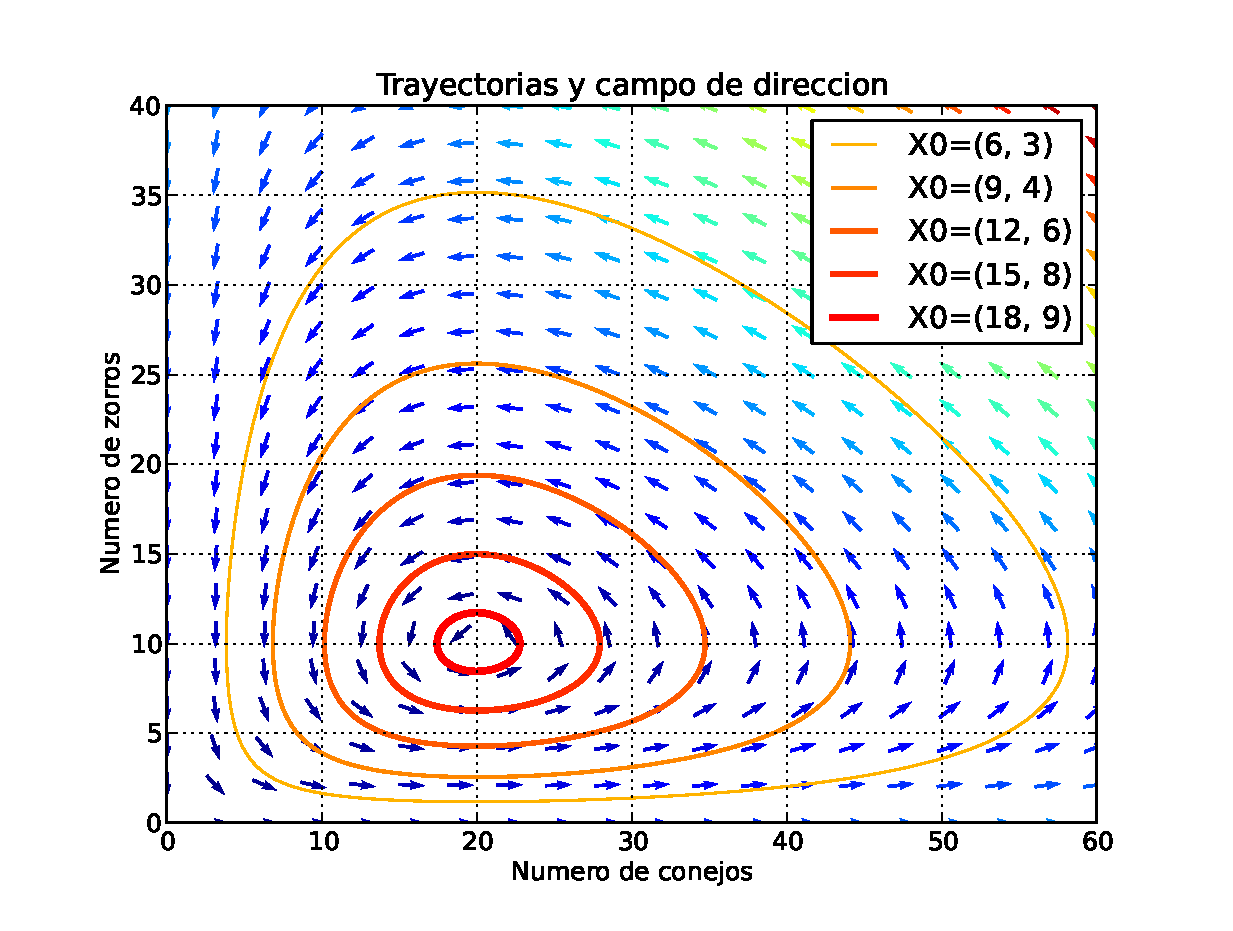
\includegraphics[scale=0.5]{LotkaVolterra_02.eps} 
% \end{figure}
% \end{frame}
% \begin{frame}
% \frametitle{Ejercicio para resolver}
% El modelo de Lorenz se usa para estudiar la formación de torbellinos en la atmósfera, aunque abordó el problema de manera general, estableció las bases para el estudio de sistemas dinámicos.
% \end{frame}
% \begin{frame}
% \frametitle{Ejercicio para resolver}
% El conjunto de ecuaciones está dado por
% \begin{align*}
% \dfrac{dy_{1}}{dt} &= a(y_{2} - y_{1}) \\
% \dfrac{dy_{2}}{dt} &= (b - y_{3}) \: y_{1} - y_{2} \\
% \dfrac{dy_{3}}{dt} &= y_{1} \: y_{2} - c \: y_{3}
% \end{align*}
% en el modelo $a$, $b$ y $c$ son parámetros positivos. 
% \end{frame}
% \begin{frame}
% \frametitle{Ejercicio para resolver}
% Resuelve este modelo numéricamente y grafica la solución.
% \\
% \bigskip
% Utiliza los siguientes valores $a = 10$, $b = 28$ y $c =    8/3$. Interpreta la solución.
% \end{frame}
% \begin{frame}[plain]
% \frametitle{Resultado gráfico}
% \begin{figure}
%     \centering
%     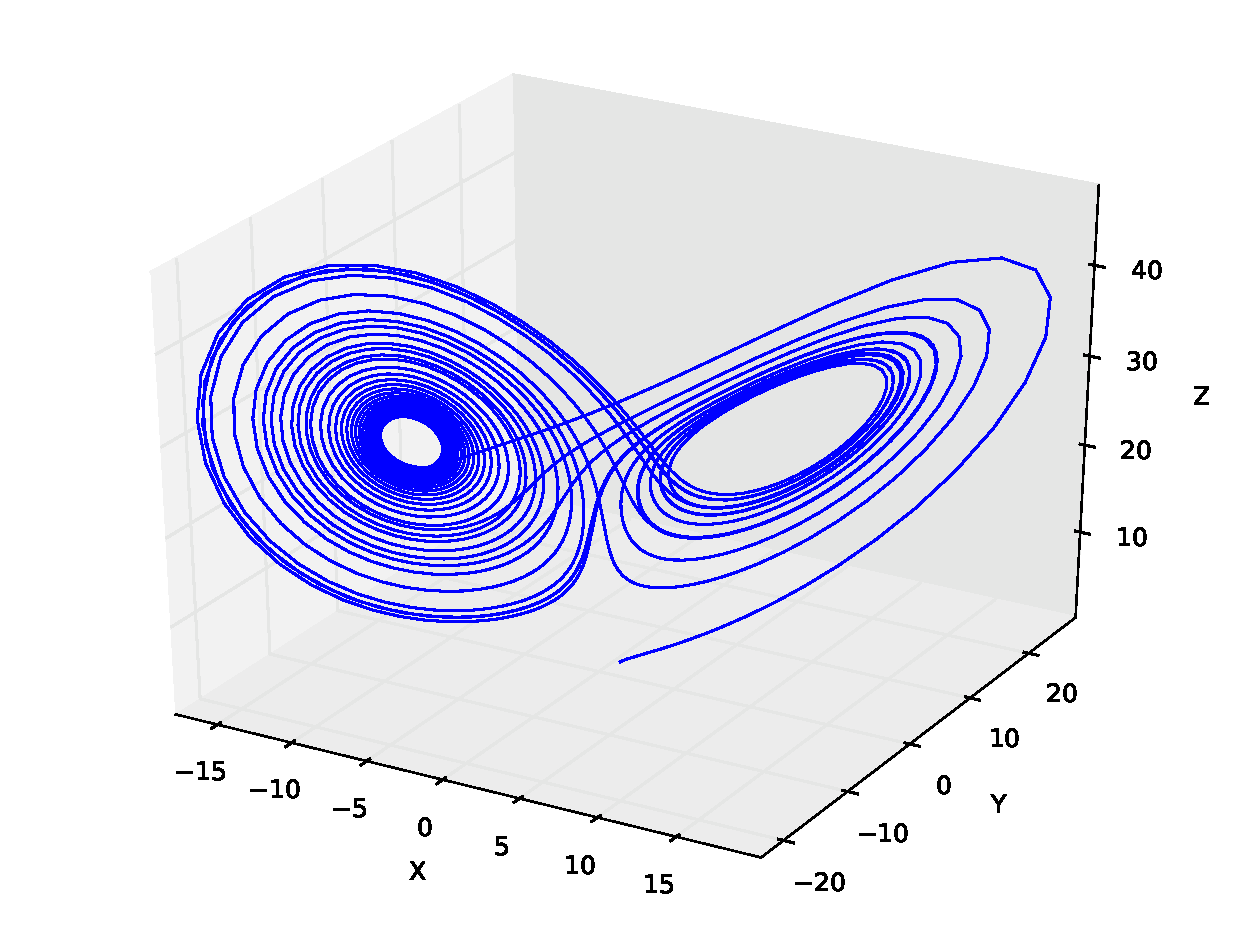
\includegraphics[scale=0.5]{Lorenz_01.eps} 
% \end{figure}
% \end{frame}
% \begin{frame}[fragile]
% \frametitle{Para generar una gráfica 3D}
% Para graficar una función de tres variables en \funcionazul{matplotlib}, debemos de utilizar una combinación de dos librerías:
% \begin{verbatim}
% import matplotlib.pyplot as plt
% import mpl_toolkits.mplot3d.axes3d as p3
% \end{verbatim}    
% \end{frame}
% \begin{frame}[fragile]
% \frametitle{Usando \texttt{plot3D}}
% Hay un importante cambio cuando graficamos tres variables con \funcionazul{matplotlib}, hay adecuar el espacio de trabajo mediante la siguiente referencia:
% \begin{verbatim}
% fig = plt.figure()

% ax = p3.Axes3D(fig)
% \end{verbatim}
% Con \texttt{plt} definimos el espacio común de graficación, pero con \texttt{ax}, ahora y contamos con la manera de usar la graficación de tres variables.
% \end{frame}
% \begin{frame}[fragile]
% \frametitle{La función \texttt{plot3D}}
% La función \funcionazul{plot3D} ocupa los argumentos de la misma manera que \funcionazul{plot}, por lo que debemos de usar la sintaxis:
% \begin{verbatim}
% ax.plot3D(x, y, z)

% ax.set_xlabel('X')
% ax.set_ylabel('Y')
% ax.set_zlabel('Z')

% fig.add_axes(ax)
% plt.show()
% \end{verbatim}
% \end{frame}

\end{document}